\documentclass[12pt,oneside]{article}
\usepackage[utf8]{inputenc}
\usepackage[american]{babel}
\usepackage{bookmark}
\usepackage{microtype}
\usepackage{setspace}
  \setstretch{1.15}
\usepackage[style=authoryear,sorting=nyt,backend=biber,
  hyperref=true,abbreviate=true,
  maxcitenames=1,maxbibnames=1]{biblatex}
  \renewbibmacro{in:}{}
  \addbibresource{../main.bib}
\usepackage{xcolor}
  \definecolor{dgreen}{RGB}{62,100,62}
  \definecolor{lgreen}{RGB}{249,255,249}
  \pagecolor{lgreen}
\usepackage{graphicx}
\usepackage{hyperref}
  \hypersetup{colorlinks=true,allcolors=blue!40!black}
\setlength{\topskip}{6pt}
\setlength{\parskip}{6pt} % before par

\DeclareCiteCommand{\citea}
  {\boolfalse{citetracker}\boolfalse{pagetracker}\usebibmacro{prenote}}
  {\href{\thefield{url}}{\printnames{labelname}}}
  {\multicitedelim}
  {\usebibmacro{postnote}}

\def\zoldversion{0.2.4}

\title{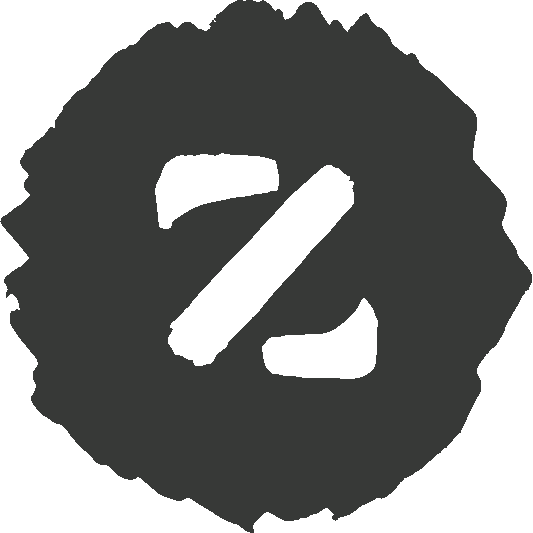
\includegraphics[scale=0.3]{../images/logo.pdf}\\
  Zold: A New Cryptocurrency\\
  {\small\colorbox{dgreen}{\color{lgreen}{Green Paper}}}}
\author{Yegor Bugayenko\\
  \texttt{yegor256@gmail.com}\\
  \href{https://www.zold.io}{\texttt{www.zold.io}}\\[1em]
  \href{https://github.com/zold-io/papers/releases/tag/\zoldversion}{\texttt{\zoldversion}}}

\begin{document}
\raggedbottom

\maketitle

In the last few years digital currencies have successfully demonstrated
their ability to become alternative financial instruments in many
different markets. Most of the technologies available at the moment are
based on the principles of \href{https://en.wikipedia.org/wiki/Blockchain}{Blockchain} architecture, including
dominating currencies like \href{https://bitcoin.org/}{Bitcoin} and
\href{https://ethereum.org/}{Ethereum}. Despite its
popularity, Blockchain is not the best possible solution for all scenarios.
One such example is for fast micro-payments.
\href{https://www.zold.io}{Zold} is an experimental alternative
that enables distributed transactions between
anonymous users, making micro-payments financially feasible and fast.
It borrows the ``\href{https://en.wikipedia.org/wiki/Proof-of-work_system}{proof of work}'' principle from Bitcoin,
and suggests a different architecture for digital wallet maintenance,
explained in detail in the \href{https://papers.zold.io}{White Paper}.

\pagebreak

\section*{The Market}

Since its release in 2009, \href{https://bitcoin.org/}{Bitcoin} from
``a libertarian fairy tale'' and ``a simple Silicon Valley exercise in hype''
turned into ``a catalyst to reshape the financial system in ways that are more
powerful for individuals and businesses alike,'' according to \citea{andreessen2014}.
Even though \citea{cheah2015} argues that
``the fundamental value of Bitcoin is zero,''
it seems that ``the question is not whether Bitcoin has value; it already does,''
according to \citea{van2014}.
``The question is whether the efficiencies of a cybercurrency
like Bitcoin can be merged with the certainties of an honest central bank.''

The core component of Bitcoin is Blockchain technology, which
``ensures the elimination of the double-spend problem, with the help
of public-key cryptography'' and ``coins are transferred by the
digital signature of a hash,''
explains \citea{pilkington2016}.
Very soon after \href{https://bitcoin.org/}{Bitcoin} was created, similar products were introduced,
which were also based on the principles of Blockchain, such as
\href{https://ethereum.org/}{Ethereum} by \citea{buterin2013}.

Even though Blockchain is a sound solution to the
\href{https://en.wikipedia.org/wiki/Double-spending}{double-spending problem},
there could be other solutions,
including different ``proof-of-x'' alternatives.
For example, \citea{everaere2010} gave
a summary of them and introduced their own,
\citea{boyen2016} described
``a truly distributed ledger system based on a lean graph of cross-verifying transactions,''
recently \href{https://www.iota.org/}{IOTA}, a ``tangle-based cryptocurrency,'' was launched by
\citea{popov2017},
\citea{hashgraph} claims to be ``the world's first mass-adopted public distributed ledger'',
and so on.

\pagebreak

\section*{The Problems}

Zold is also a decentralized digital currency that maintains its ledgers
through an unpredictable amount of anonymous and untrustable server nodes, trying to guarantee
data consistency. The architecture of Zold is not Blockchain-based.
The development of Zold was motivated by the desire to overcome
two obvious disadvantages present in the majority of cryptocyrrencies:

The first problem is that transaction processing is rather slow.
\href{https://goo.gl/sWiAWc}{The current rate} for \href{https://bitcoin.org/}{Bitcoin}
processing speed is 7 transactions per second (tps)
while Paypal handles an average of 115 tps and the VISA
network has a peak capacity of 47,000 tps.
\citea{karame2012} says that
``Bitcoin requires tens of minutes to verify a transaction
and is therefore inappropriate for fast payments.''
It is inevitable, since
``processing speed is at odds with the security aspects of the underlying
proof-of-work based consensus mechanism'' according
to \citea{kiayias2015}.
\href{https://ethereum.org/}{Ethereum}, according to \citea{fekkes2018}, can process
``two times more transactions per second than Bitcoin is able to do,''
but this still is rather slow.

The second problem, as noted by \citea{popov2017},
is that ``it is not easy to get rid
of fees in the blockchain infrastructure since they serve
as an incentive for the creators of blocks.''
\citea{moser2015} says that ``Bitcoin users are encouraged to
pay fees to miners, up to 10 cents (of USD) per transaction, irrespective of the
amount paid'' which especially hurts when transaction amounts are smaller than a dollar.
Moreover, according to \citea{kaskaloglu2014},
``an increase in transaction fees of Bitcoin is inevitable.''

Thus, the speed is low and the processing fees are high.
Zold was created as an attempt to resolve these two problems
by specifically focusing on micro payments.

\pagebreak

\section*{The Features}

First, unlike all other crypto currencies, there is no central ledger in Zold.
Each wallet has its own personal ledger.
All transactions in each ledger are confirmed by
\href{https://en.wikipedia.org/wiki/RSA_(cryptosystem)}{RSA} signatures of their owners.
This enables high scalability and performance.

Second, similar to many other digital currencies, including
\href{https://bitcoin.org/}{Bit\-coin},
\href{https://ethereum.org/}{Eth-reum},
\href{https://getmonero.org/}{Mone\-ro},
\href{https://plancoin.co/}{Plancoin},
\href{https://dero.io/}{Dero},
and many others, Zold nodes find consensus by using the CPU power to perform certain expensive and meaningless calculations
that result in finding hash suffixes, also known as ``proof-of-work,''
initially introduced by \citea{back1997} in \citeyear{back1997}.
This guarantees data consistency and eliminates the possibility of double-spending.

Third, Zold is a pre-mined digital asset, similar to
\href{https://ripple.com/}{Ripple},
\href{https://www.cardano.org/en/home/}{Cardano},
\href{https://www.stellar.org/}{Stellar},
\href{https://neo.org/}{NEO}, and many others.
Zold algorithmically limits its total supply, which is 2,15 billion ZLD.
To compare, the total supply of some other currencies is:
21m in \href{https://bitcoin.org/}{Bitcoin},
100b in \href{https://ripple.com/}{Ripple},
84m in \href{https://litecoin.org/}{Litecoin},
and
19m in \href{https://www.dash.org/}{Dash}.
\citea{bohr2014} explains that cryptocurrencies limit their
total suply in order ``to protects against inflationary forces,''
so does Zold in order to protect its market value.

Fourth, the speed of transaction processing in Zold
literally has no limits, because all payments are made locally, on users'
machines and then pushed to the network for merging and storing.

Fifth, the cost of transaction processing
is lower than what most other payment systems can offer. To process
a thousand transactions a user has to pay (approximately) \$500 in Bitcoin, \$300 in \href{https://ethereum.org/}{Ethereum},
\$45 in \href{https://litecoin.org/}{Litecoin}, \$12 in \href{https://ripple.com/}{Ripple}, and \$9 in Bitcoin Cash.
In Zold it is as little as \$4, which makes it one of the most cost effective
cryptocurrencies.

\pagebreak

\section*{The Roadmap}

Zold is a \href{https://github.com/zold-io}{GitHub}-hosted open source
software product, just like most other cryptocurrencies.
Its first experimental version was created and launched by \href{https://www.yegor256.com}{Yegor Bugayenko},
the CEO of \href{https://www.zerocracy.com}{Zerocracy}, on May~27, 2018.
A distributed \href{http://www.zold.io/map.html}{network of nodes},
which are running Zold software, is maintained by
anonymous volunteers. The development of further versions and the
maintenance of existing ones depends on the activity of GitHub
contributors, partially sponsored by \href{https://www.zerocracy.com}{Zerocracy, Inc.}

Just like \href{https://www.sec.gov/}{SEC} chairman Jay Clayton
\href{https://www.cnbc.com/video/2018/06/06/sec-chairman-cryptocurrencies-like-bitcoin--not-securities.html}{recently mentioned},
``cryptocurrencies like Bitcoin are not securities.''
Similar to Bitcoin and Ethereum, ZLD is a cryptocurrency, not a security.
It is distributed by Zerocracy as a digital gift to those who
actively contribute to Zerocracy ecosystem, the development of Zold software,
and the maintenance of nodes.

Aside from programming, Zold enthusiasts may contribute their monetary assets,
like US dollars, to any project managed by Zerocracy.
In exchange, they get rewarded with ZLD digital coins.
Later, they are able to trade their ZLD coins to other digital currencies
and fiat money, through exchanges or directly.

It is assumed that the market price of ZLD will grow due to its technical
advantages and the popularity of Zerocracy platform among programmers
and software companies.

\end{document}
